\subsection{Segitiga}
Pada segitiga $ABC$ seperti gambar berikut:
\begin{center}
\begin{tikzpicture}
    % Define the coordinates of the vertices
    \coordinate (A) at (0,0);
    \coordinate (B) at (8,0);
    \coordinate (C) at (1.5,4);
    
    % Draw the triangle
    \draw (A) -- (B) -- (C) -- cycle;
    
    % circumcircle
    \tkzCircumCenter(A,B,C)\tkzGetPoint{O}
    \tkzDrawPoint(O)
    \tkzDrawCircle(O,A)
    
    % incircle
    \tkzDefCircle[in](A,B,C)\tkzGetPoint{I}\tkzGetLength{rIN}
    \tkzDrawPoint(I)
    \tkzDrawCircle[R](I,\rIN pt)
    
    % angle bisector
    \tkzDrawBisector[blue](B,A,C)\tkzGetPoint{E}
    \tkzDrawCircle[R](E,1 pt)
    
    %altitude
    \tkzDefPointBy[projection=onto B--C](A) \tkzGetPoint{D}
    \tkzDefPointBy[projection=onto B--A](C) \tkzGetPoint{C1}
    \tkzInterLL(A,D)(C,C1) \tkzGetPoint{H}
    \tkzDrawPoints(H) \tkzLabelPoints[below right](H)
    \tkzDrawSegment[red](A,D)
    \tkzDrawSegment[red](C,C1)

    %garis sumbu
    \tkzDefPointBy[projection=onto B--C](O) \tkzGetPoint{M}
    \tkzDefPointBy[homothety=center O ratio 3.2](M) \tkzGetPoint{M1}
    \tkzDefPointBy[homothety=center O ratio -3.2](M) \tkzGetPoint{M2}
    \tkzDrawSegment(M1,M2)
    \tkzDefPointBy[projection=onto B--A](O) \tkzGetPoint{M3}

    %centroid
    \tkzDrawSegment[green](A,M)
    \tkzDrawSegment[green](C,M3)
    \tkzInterLL(A,M)(C,M3) \tkzGetPoint{G}
    \tkzDrawPoints(G) \tkzLabelPoints[below right](G)
    
    % Label the vertices
    \node[below left] at (A) {$A$};
    \node[below right] at (B) {$B$};
    \node[above] at (C) {$C$};
    \node[below right] at (I) {$I$};
    \node[right] at (O) {$O$};
    \node[above right] at (E) {$E$};
    \node[above] at (D) {$D$};
    \node[right] at (M) {$M$};
\end{tikzpicture}
\end{center}
\begin{enumerate}
    \item Garis bagi $AE$ yaitu garis yang membagi dua sudut $A$ sama besar sehingga $\angle BAE = \angle EAC$. 
    \item Garis berat $AM$ dengan $M$ adalah titik tengah $BC$.
    \item Garis tinggi $AD$ adalah garis yang tegak lurus dengan $BC$. $D$ biasa disebut dengan proyeksi $A$ ke $BC$.
    \item Garis $OM$ adalah salah satu garis sumbu segitiga $ABC$, yaitu garis yang melewati titik tengah sisi segitiga dan tegak lurus dengan sisi itu.
    \item Pertemuan atau perpotongan ketiga garis tinggi segitiga $ABC$ adalah titik tinggi, dalam gambar ini adalah $H$ (orthocenter).
    \item Pertemuan atau perpotongan ketiga garis bagi segitiga $ABC$ adalah titik bagi atau titik pusat lingkaran dalam (incircle) segitiga $ABC$ dalam gambar ini adalah $I$ (incenter).
    \item Pertemuan atau perpotongan ketiga garis berat segitiga $ABC$ adalah titik berat (centroid).
    \item Pertemuan atau perpotongan ketiga garis sumbu segitiga $ABC$ adalah titik pusat lingkaran luar (circumcircle) segitiga $ABC$ yang dalam gambar ini adalah $O$ (circumcenter).
    \item Berlaku \textbf{ketaksamaan segitiga} yaitu $AB+BC>CA$, $BC+CA>AB$, dan $CA+AB>BC$. Selain itu juga berlaku $|AB-BC|<CA$, $|BC-CA|<AB$, dan $|CA-AB|<BC$.
\end{enumerate}
\subsection{Kesebangunan Segitiga}
\begin{center}
\begin{tikzpicture}
  % First triangle
  \coordinate (A) at (0,0);
  \coordinate (B) at (3,0);
  \coordinate (C) at (2,2);
  \draw (A) -- (B) -- (C) -- cycle;

  % Second triangle
  \coordinate (D) at (6,0);
  \coordinate (E) at (12,0);
  \coordinate (F) at (8,4);
  \draw (D) -- (E) -- (F) -- cycle;

  % Labeling the vertices
  \node[below] at (A) {$A$};
  \node[below] at (B) {$B$};
  \node[above] at (C) {$C$};
  \node[below] at (D) {$D$};
  \node[below] at (E) {$E$};
  \node[above] at (F) {$F$};

  \draw pic[draw=green!30,fill=green!30,angle radius=0.5cm] {angle=A--C--B};
  \draw pic[draw=green!30,fill=green!30,angle radius=0.5cm] {angle=D--F--E};
  \draw pic[draw=red!30,fill=red!30,angle radius=0.5cm] {angle=B--A--C};
  \draw pic[draw=red!30,fill=red!30,angle radius=0.5cm] {angle=F--E--D};
  \draw pic[draw=blue!30,fill=blue!30,angle radius=0.5cm] {angle=C--B--A};
  \draw pic[draw=blue!30,fill=blue!30,angle radius=0.5cm] {angle=E--D--F};
\end{tikzpicture}
\end{center}



Segitiga $ABC$ dan $DEF$ sebangun atau $ABC \sim DEF$ jika dan hanya jika minimal salah satu syarat ini terpenuhi:
\begin{enumerate}
    \item $\angle ABC = \angle DEF$ dan $\angle BAC = \angle EDF$.
    \item $\dfrac{AB}{DE} = \dfrac{BC}{EF} = \dfrac{CA}{FD}$.
    \item $\dfrac{AB}{DE} = \dfrac{BC}{EF}$ dan $\angle ABC = \angle DEF$ (sudut yang diapit dua sisi yang diperbandingkan nilainya sama)
\end{enumerate}

\subsection{Kekongruenan Segitiga}
\begin{center}
\begin{tikzpicture}
  % First triangle
  \coordinate (A) at (0,0);
  \coordinate (B) at (3,0);
  \coordinate (C) at (2,2);
  \draw (A) -- (B) -- (C) -- cycle;

  % Second triangle
  \coordinate (D) at (6,0);
  \coordinate (E) at (9,0);
  \coordinate (F) at (7,2);
  \draw (D) -- (E) -- (F) -- cycle;

  % Labeling the vertices
  \node[below] at (A) {$A$};
  \node[below] at (B) {$B$};
  \node[above] at (C) {$C$};
  \node[below] at (D) {$D$};
  \node[below] at (E) {$E$};
  \node[above] at (F) {$F$};

  \draw pic[draw=green!30,fill=green!30,angle radius=0.5cm] {angle=A--C--B};
  \draw pic[draw=green!30,fill=green!30,angle radius=0.5cm] {angle=D--F--E};
  \draw pic[draw=red!30,fill=red!30,angle radius=0.5cm] {angle=B--A--C};
  \draw pic[draw=red!30,fill=red!30,angle radius=0.5cm] {angle=F--E--D};
  \draw pic[draw=blue!30,fill=blue!30,angle radius=0.5cm] {angle=C--B--A};
  \draw pic[draw=blue!30,fill=blue!30,angle radius=0.5cm] {angle=E--D--F};

    \tkzMarkSegment[pos=.5,mark=|](C,B)
    \tkzMarkSegment[pos=.5,mark=|](D,F)
    \tkzMarkSegment[pos=.5,mark=||](C,A)
    \tkzMarkSegment[pos=.5,mark=||](E,F)
    \tkzMarkSegment[pos=.5,mark=|||](B,A)
    \tkzMarkSegment[pos=.5,mark=|||](E,D)
\end{tikzpicture}
\end{center}

Sedangkan $ABC$ dan $DEF$ dikatakan kongruen atau $\triangle ABC \cong \triangle DEF$ jika dan hanya jika $AB=DE, BC=EF, CA=FD$ atau dengan kata lain kedua segitiga tersebut sebangun dan ada salah satu sisi dari kedua segitiga tersebut yang panjangnya sama. Simpelnya kongruen = sama persis.

\subsection{Teorema Pythaogras}
Salah satu teorema paling terkenal di kalangan awam (atau setidaknya di pop culture). Diberikan segitiga $ABC$ dengan sudut $C$ siku-siku. Jika panjang sisi $AB=c$, $BC=a$, dan $CA=b$, maka berlaku
\begin{align*}
    a^2+b^2=c^2
\end{align*}
\begin{center}
    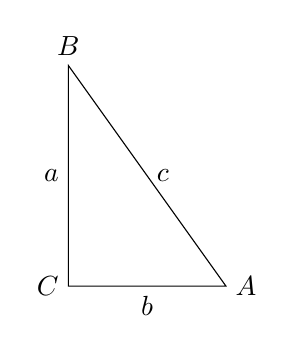
\begin{tikzpicture}
    % titik-titik segitiga
    \coordinate[label=left:$C$]  (C) at (-1.5cm,-1.cm);
    \coordinate[label=above:$B$] (B) at (-1.5cm,1.8cm);
    \coordinate[label=right:$A$] (A) at (0.5cm,-1.cm);
    
    % pembuatan segitiga
    \draw (A) -- node[right]{$c$} (B)  -- node[left]{$a$} (C) -- node[below]{$b$} cycle;
    \end{tikzpicture}
\end{center}
\subsection{Latihan Soal Pythagoras}
\begin{enumerate}
    \item (OSK SMP 2016) Diketahui $ABCD$ dan $CEGH$ adalah dua persegipanjang kongruen dengan panjang $17$ cm, dan lebar $8$ cm. Titik $E$ berada di sisi $AB$ dan $D$ berada di sisi $GH$. Titik $F$ adalah titik potong sisi $AD$ dan $EG$. Luas segiempat $EFDC$ adalah .... $cm^2$.

    \item Misalkan $ABC$ adalah segitiga lancip. Titik $D$, $E$, dan $F$ terletak pada sisi $BC$, $CA$, dan $AB$, berturut-turut, sedemikian sehingga $AD$, $BE$, dan $CF$ adalah garis tinggi segitiga $ABC$. Titik $H$ adalah titik tinggi segitiga $ABC$. Jika $DE = 8$, $DF = 15$, dan $EF = 17$, tentukan panjang $AH$.
\end{enumerate}